\chapter{Experimental Comparison of Neuromuscular and Impedance Controllers}\label{sec:nm_vs_imp}

\begin{figure}[h]
    \centering 
    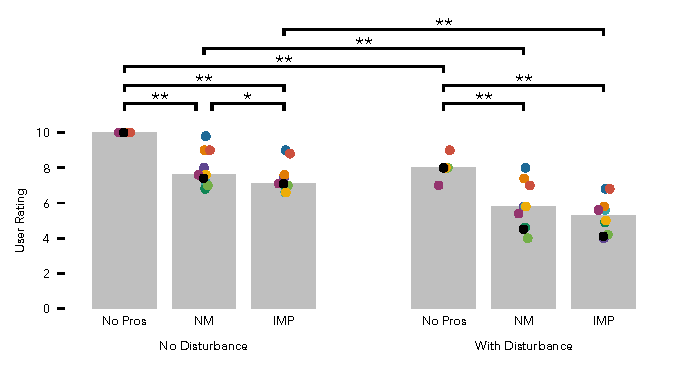
\includegraphics[width=\textwidth]{treadmill_vib_user_scores}
    \caption{Average user ratings accross all trials in both the 
    undisturbed and disturbed walking conditions when walking without the
    prosthesis (No Pros) and with the Neuromuscular (NM) prosthesis control and
    impedance (IMP) prosthesis control.}\label{fig:treadmill_user_ratings}
\end{figure}

\begin{figure}[h]
    \centering 
    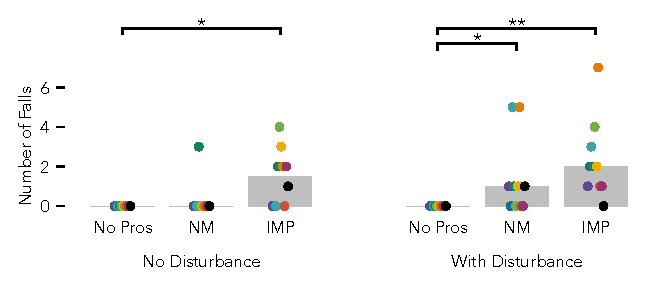
\includegraphics[width=\textwidth]{treadmill_vib_num_falls}
    \caption{Total number of falls accross all trials in both the 
    undisturbed and disturbed walking conditions when walking without the
    prosthesis (No Pros) and with the Neuromuscular (NM) prosthesis control and
    impedance (IMP) prosthesis control.}\label{fig:treadmill_exp_falls}
\end{figure}

\begin{table}[h]
  \footnotesize%
  \begin{center}
    \begin{tabular}{lcc}
      \toprule
      Fall Types & Neuromuscular & Impedance \\
      \midrule
      Fall Forward &  1 &  0 \\
      Fall Backwards &  6 &  4 \\
      Fall Left &  1 &  0 \\
      Fall Right &  0 &  3 \\
      Missed Stance / Swing Transition &  3 &  0 \\
      Missed Stance 2 / Stance 3 Transition &  0 &  7 \\
      Knee Collapse & 0 & 15 \\
      Swing Trip & 4 & 12 \\
      \bottomrule
    \end{tabular}
  \end{center}
  \caption{Tally of observed reasons for falls accross all subjects and accross
  both the undisturbed and disturbed walking conditions. Falls were manually
  classified based on video and logged prosthesis data. An indivicual Fall can
  be assigned more than one reason.}\label{tab:treadmill_exp_fall_reasons}
\end{table}

\begin{figure}[h]
    \centering 
    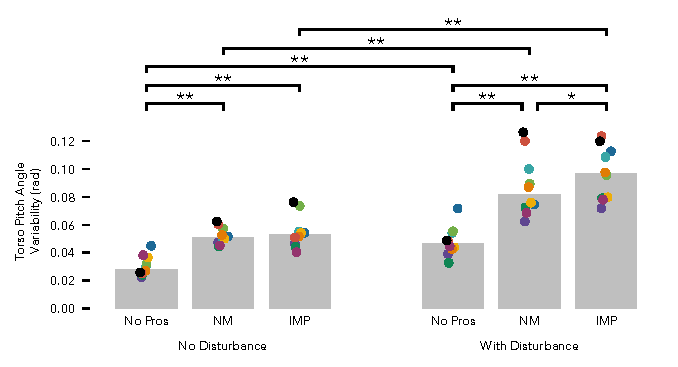
\includegraphics[width=\textwidth]{treadmill_vib_torso_var_x}
    \caption{Torso pitch angle variation. Angle variation calculated as the
    inter quartile range of torso angles after the median torso angle trajectory
    over the strides in a trial is subtracted out. For the prosthesis trials, we
    report the average variation accross the five trials for each condition.
    Grey bars show median accross subjects.}\label{fig:treadmill_exp_falls}
\end{figure}

\begin{figure}[h]
    \centering 
    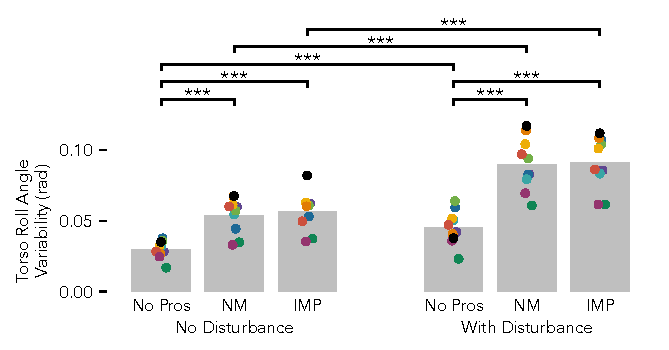
\includegraphics[width=\textwidth]{treadmill_vib_torso_var_y}
    \caption{Torso roll angle variation. Angle variation calculated as the inter
    quartile range of torso angles after the median torso angle trajectory over
    the strides in a trial is subtracted out. For the prosthesis trials, we
    report the average variation accross the five trials for each condition.
    Grey bars show median accross subjects.}\label{fig:treadmill_exp_falls}
\end{figure}
